\section{Pengenalan Anaconda}
Anaconda merupakan sebuah software yang mendistribusikan bahasa pemrograman python dan R untuk keperluan komputasi ilmiah seperti data science, machine learning, data processing skala-luas, analisis prediksi, dan lain sebaginya.
Anaconda memiliki anaconda navigator yang didalamnya terdapat software-software yang dapat digunakan untuk membuat program python dan R. Salah satu software yang akan kita gunakan yaitu Spyder. Sebelum kita membuat program kita harus menginstal anaconda terlebih dahulu.
Instalasi pada kali ini menggunakan 2 sistem operasi yaitu Windows 10 x64 dan Ubuntu 19.04. Hal yang dibutuhkan adalah laptop dengan os windows atau ubuntu dan internet.
\subsection{Instalasi Anaconda 3 Windows 10 x64}
Hal yang harus diperhatikan sebelum melakukan instalasi \textit{Anaconda Python}
\begin{enumerate}
 \item \textit{Download Anaconda Python} \\ \url{https://www.anaconda.com/distribution/}
 \item Perhatikan versi dari sistem operasi yang digunakan (versi 32bit atau 64bit)
 \item Download file anaconda yang sesuai dengan versi sistem operasi (32bit atau 64bit)
\end{enumerate}

Berikut langkah-langkah instalasi anaconda.
\begin{enumerate}
\item Buka aplikasi \textit{installer Anaconda} yang telah didwonload lalu akan muncul  gambar \ref{langkah1}, lalu pilih run untuk menjalankan proses instalasi. 
\begin{figure}[H]
        \centerline{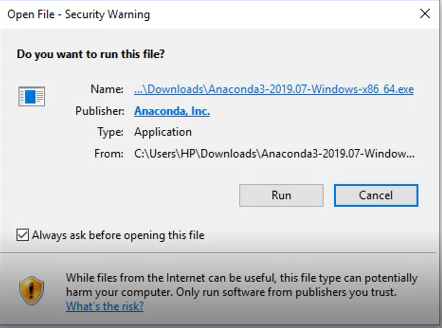
\includegraphics[scale=0.75]{figures/1}}
        \caption{Run Setup Anaconda}
		\label{langkah1}
\end{figure}

\item Tunggu hingga \textit{setup loading} selesai seperti pada gambar \ref{langkah2}.
\begin{figure}[H]
        \centerline{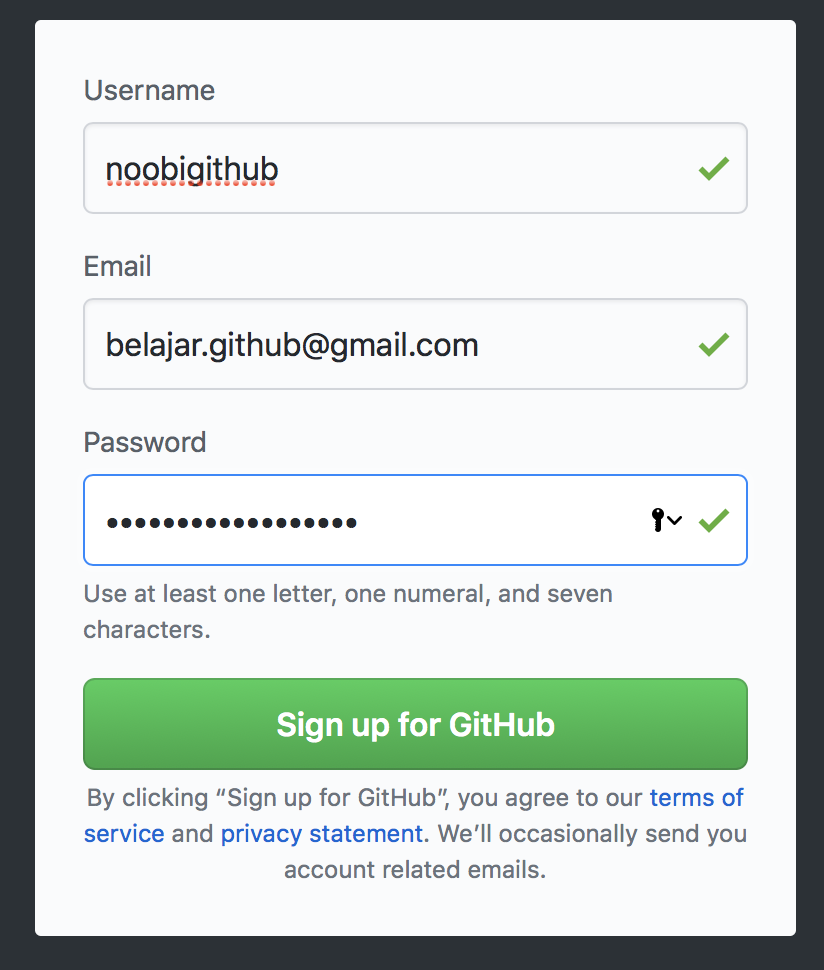
\includegraphics[scale=0.75]{figures/2}}
        \caption{Setup Loading}
		\label{langkah2}
\end{figure}

\item Jika \textit{setup loading} telah selesai, maka klik \textit{next} seperti pada gambar \ref{langkah3}.
\begin{figure}[H]
        \centerline{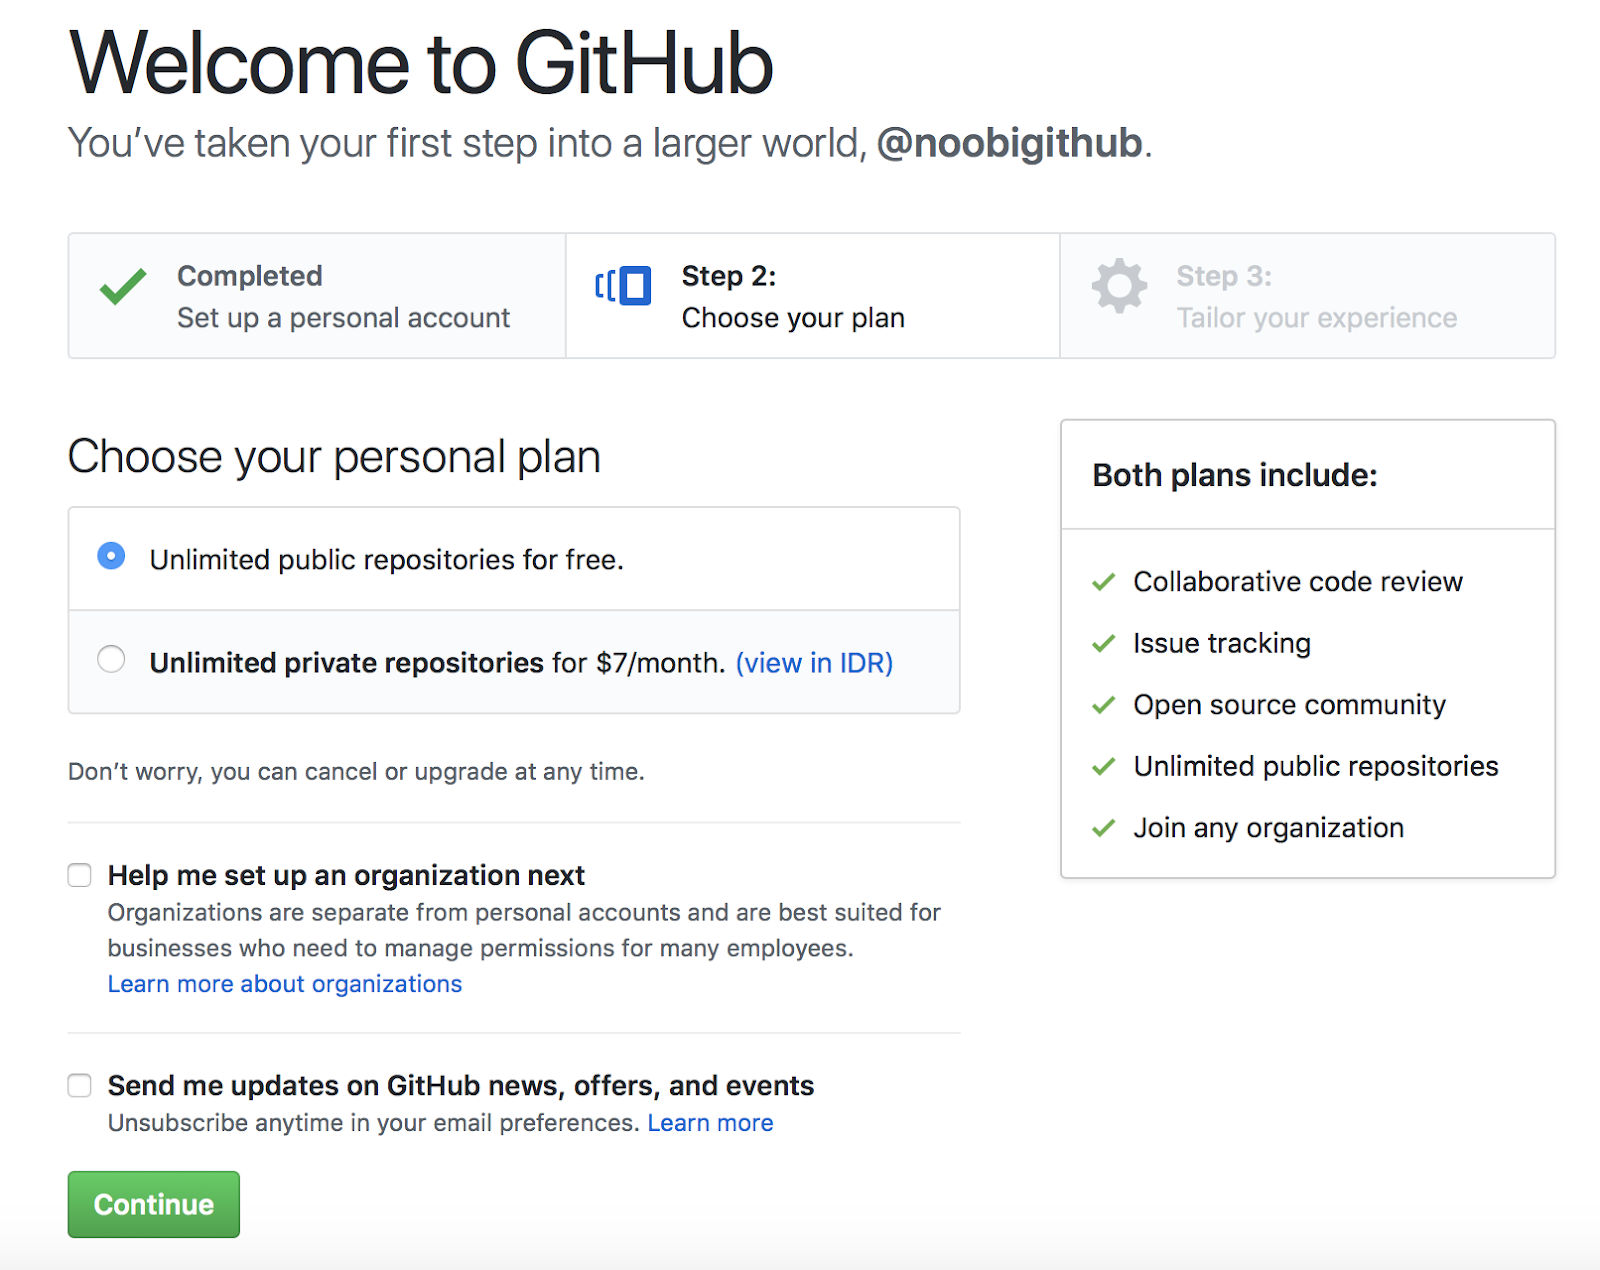
\includegraphics[scale=0.75]{figures/3}}
        \caption{Welcome to Anaconda Setup}
		\label{langkah3}
\end{figure}

\item Pada \textit{License Agreement} klik \textit{I Agree} karena jika teman-teman tidak menyetujui lisensi anaconda maka teman-teman tidak akan bisa melanjutkan proses instalasi. lakukan langkah ini seperti pada gambar \ref{Figureanaconda3}

\begin{figure}[H]
    \centering
    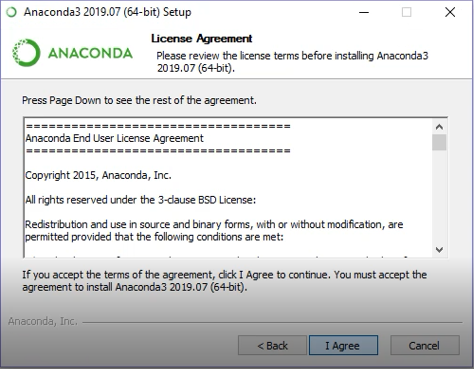
\includegraphics[scale=0.75]{figures/4}
    \caption{\textit{License Agreement}}
    \label{Figureanaconda3}
\end{figure}


\item Kemudian pilih \textit{Just Me(Recomended)} agar sesuai dengan komputer yang digunakan, kemudian klik \textit{next} seperti pada gambar \ref{Figureanaconda4}.

\begin{figure}[H]
    \centerline{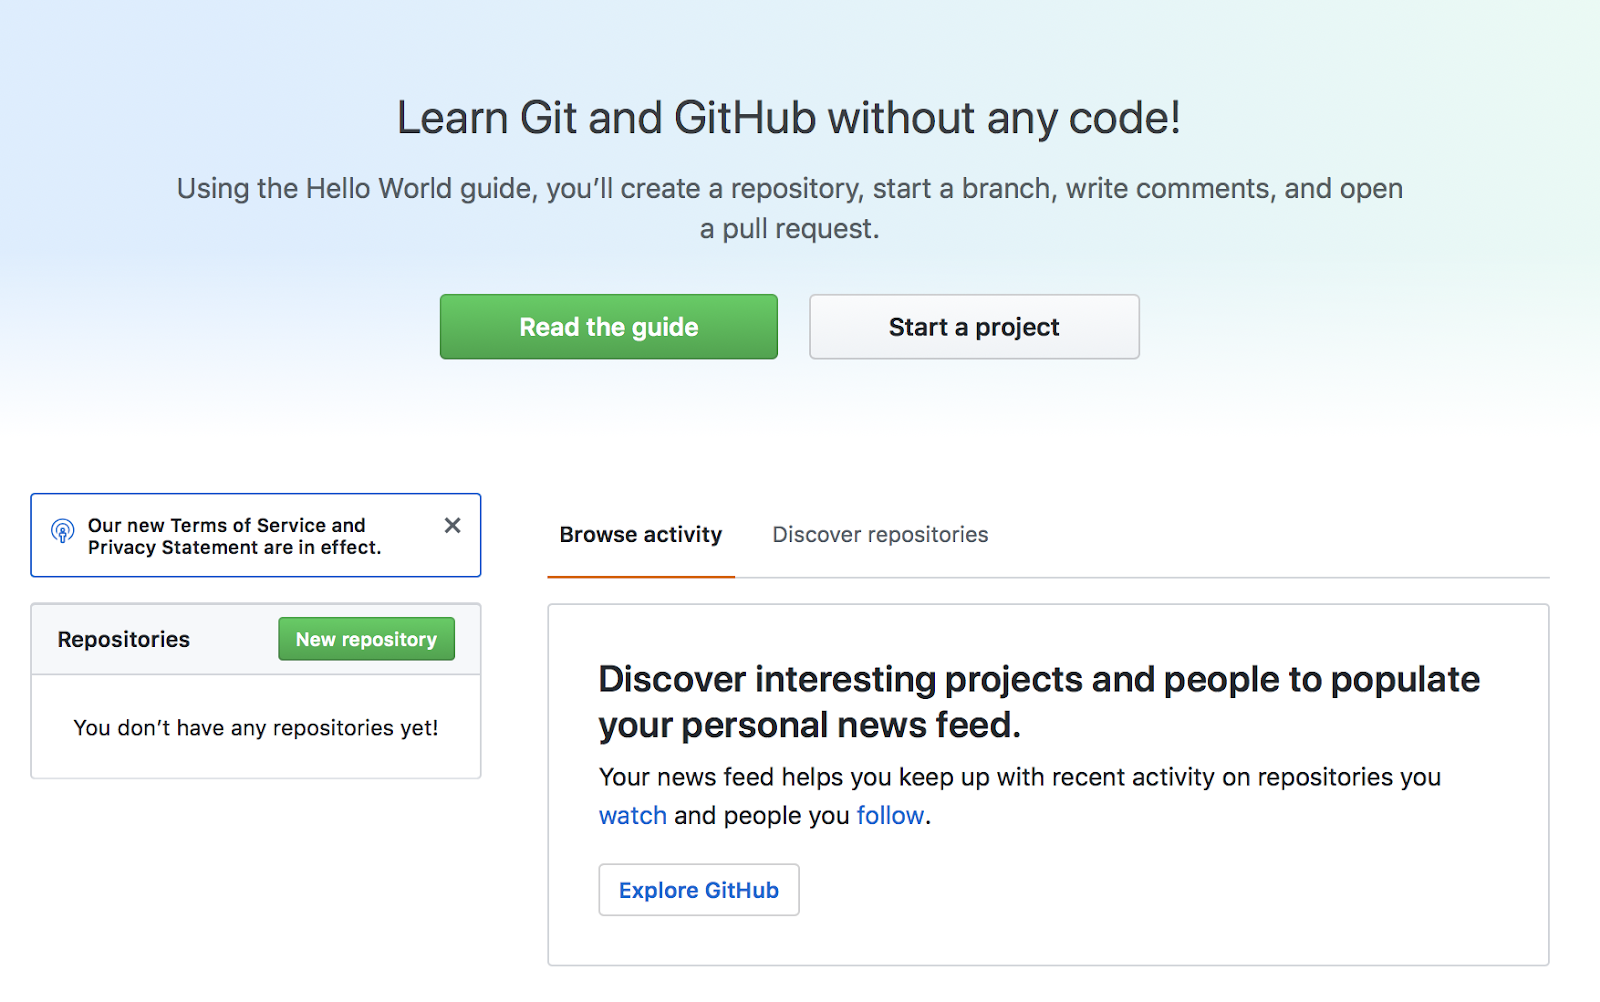
\includegraphics[scale=0.75]{figures/5}}
    \caption{\textit{Just Me(recomended)}}
    \label{Figureanaconda4}
\end{figure}


\item Kemudian pilih directori tempat kita akan \textit{menginstall anaconda} seperti pada gambar \ref{Figureanaconda5}

\begin{figure}[H]
    \centering
    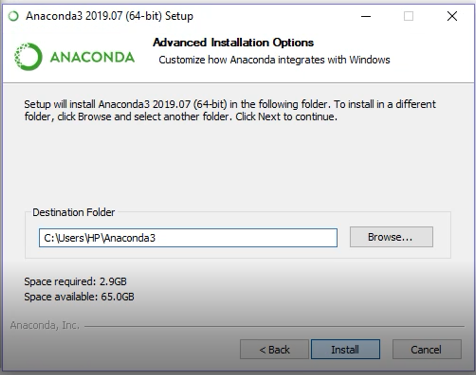
\includegraphics[scale=0.75]{figures/6}
    \caption{\textit{Pilih lokasi}}
    \label{Figureanaconda5}
\end{figure}

\item Kemudian centang \textit{Add Anaconda to my Path environtment variable}, agar saat melakukan instalasi  \textit{package anaconda, package} tersebut akan langsung tertuju ke \textit{path anaconda} tidak ke aplikasi yang lain. kemudian Klik \textit{install} seperti pada gambar \ref{Figureanaconda6}.

\begin{figure}[H]
    \centering
    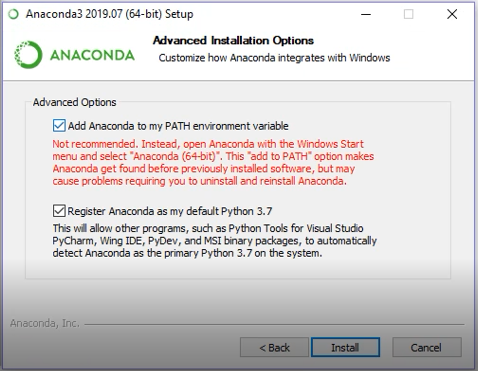
\includegraphics[scale=0.75]{figures/7}
    \caption{\textit{Centang Anaconda to my PATH}}
    \label{Figureanaconda6}
\end{figure}

\item Tunggu sampai proses \textit{installasi} selesai seperti pada gambar \ref{Figureanaconda7}.

\begin{figure}[H]
    \centering
    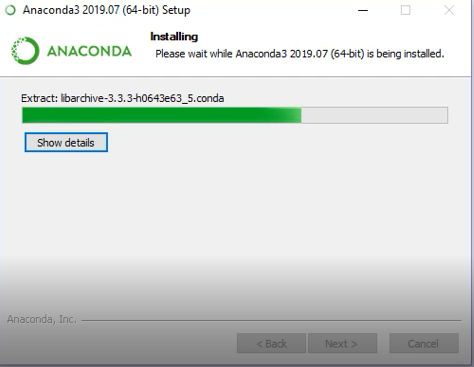
\includegraphics[scale=0.75]{figures/8}
    \caption{\textit{Waiting Installation Complete}}
    \label{Figureanaconda7}
\end{figure}

\item Apabila instalasi telah selesai  maka akan terlihat seperti gambar \ref{Figureanaconda8}, kemudian klik \textit{next}
\begin{figure}[H]
    \centering
    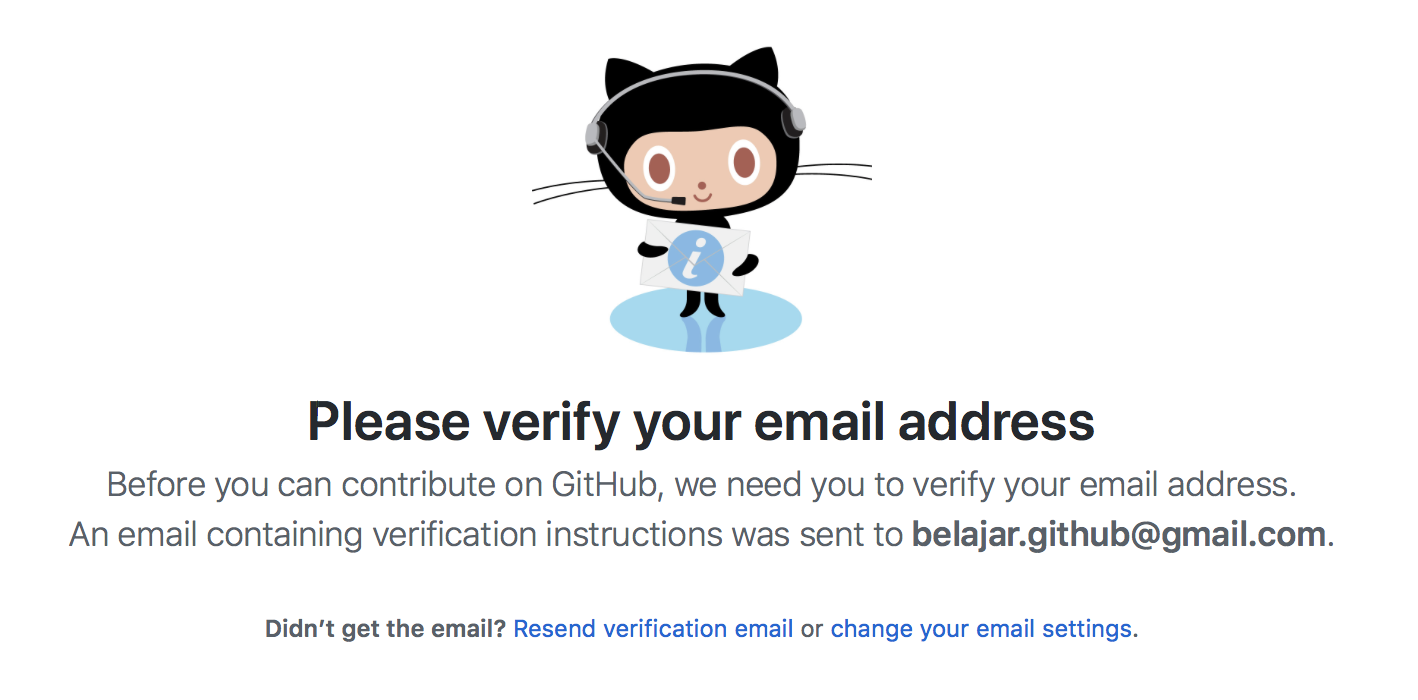
\includegraphics[scale=0.75]{figures/9}
    \caption{\textit{Installation Complete}}
    \label{Figureanaconda8}
\end{figure}

\item apabila muncul gambar \ref{Figureanaconda70}, maka klik \textit{next}
\begin{figure}[H]
    \centering
    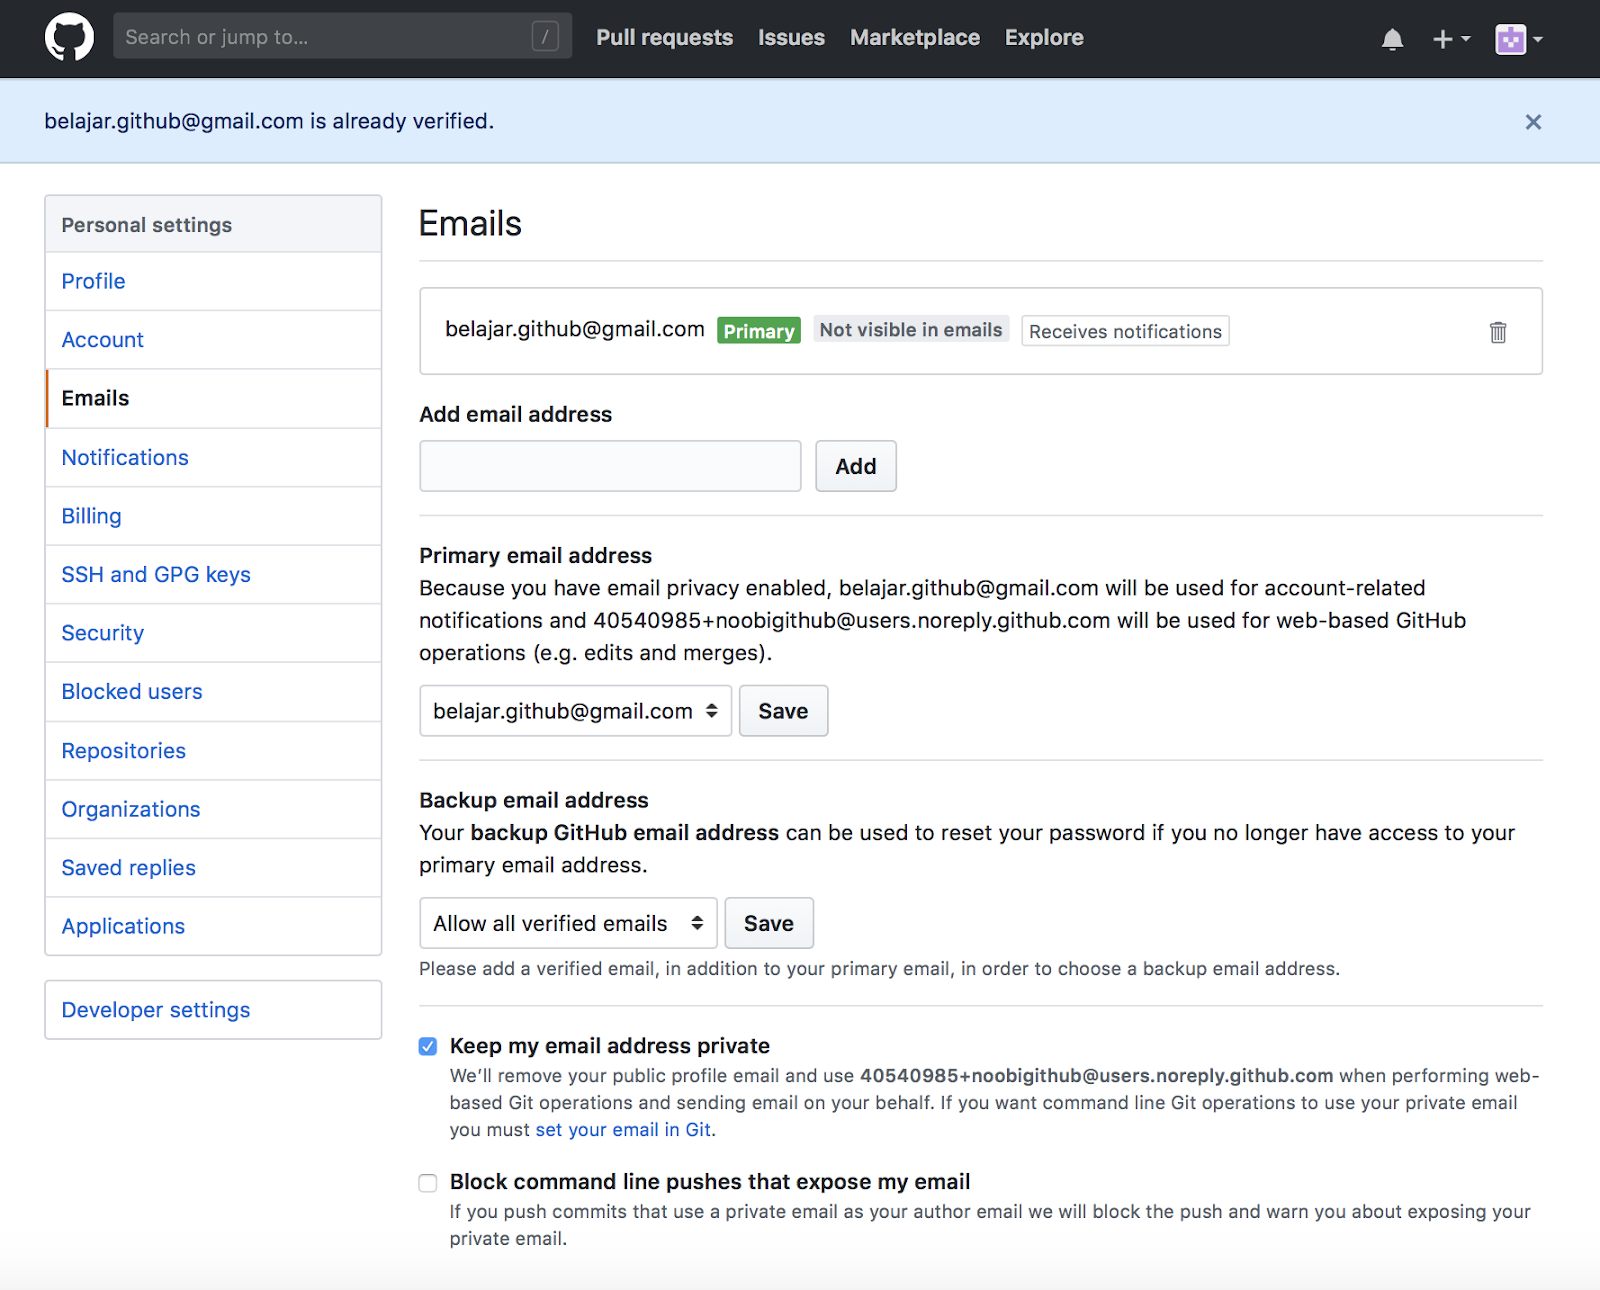
\includegraphics[scale=0.75]{figures/10}
    \caption{\textit{Anaconda+JetBrains}}
    \label{Figureanaconda70}
\end{figure}

\item Jika instalasi telah selesai maka akan ada ucapan terima kasih telah menginstall anaconda 3 seperti pada gambar \ref{Figureanaconda9}, hal ini menandakan bahwa teman-teman telah selesai dan berhasil melakukan instalasi anaconda. Kemudian klik \textit{finish} untuk mengakhiri instalasi.

\begin{figure}[H]
    \centering
    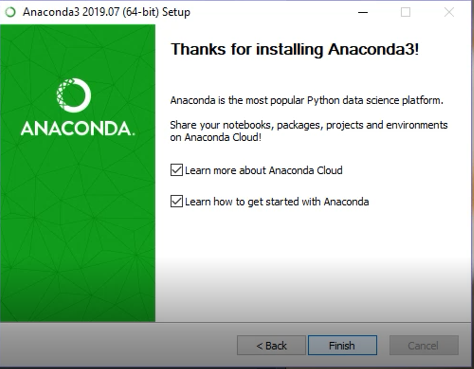
\includegraphics[scale=0.75]{figures/11}
    \caption{\textit{Thanks for install Anaconda}}
    \label{Figureanaconda9}
\end{figure}
\end{enumerate}

\subsection{Update Anaconda dan Spyder}
Kenapa kita harus melakukan update anaconda dan spyder? melakukan update diperlukan agar software yang kita gunakan merupakan software yang terbaru, karena versi lama dan versi baru akan memiliki banyak perbedaan dan akan menjadi masalah nantinya ketika kita membuat program atau mengimportkan modul-modul python yang digunakan.
Berikut cara mengupdate Spyder:
\begin{enumerate}
\item Buka anaconda prompt, lalu ketikkan perintah conda update spyder
\item Konfirmasi update dengan mengetikkan y, lalu tekan enter
\item Tunggu hingga installan selesai
\end{enumerate}
Berikut cara mengupdate Anaconda:
\begin{enumerate}
\item Buka anaconda prompt, lalu ketikkan perintah conda update anaconda
\item Konfirmasi update anaconda dengan mengetikkan y dan kemudian tekan enter
\item Tunggu hingga installan selesai
\end{enumerate}

\subsection{Instalasi Anaconda Ubuntu 19.04}
Ikuti langkah berikut untuk instalasi python pada Ubuntu 19.04:
\begin{enumerate}
\item Pertama kita kunjungi situs \\ \textbf{\textit{\url{https://www.anaconda.com/distribution/}\#download-section}} seperti gambar ~\ref{anacondadownload} dan pilih \textbf{64-Bit (x86) Installer (517 MB)}
\begin{figure}[H]
\centering
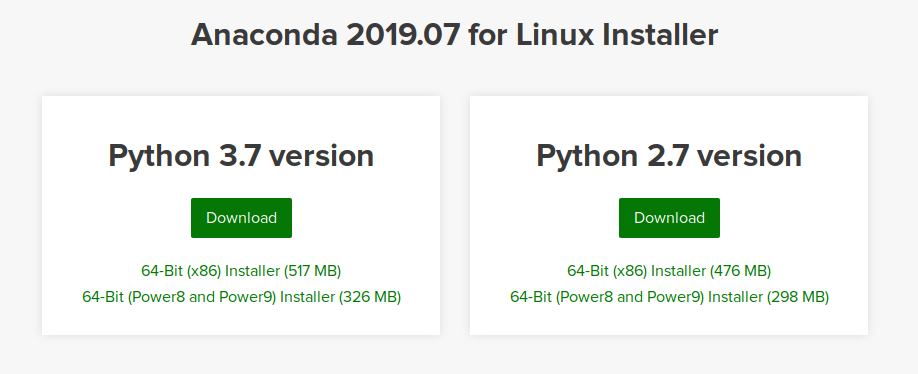
\includegraphics[width=1\textwidth]{figures/ubuntu/anacondadownload.png}
\caption{Gambar halaman download}
\label{anacondadownload}
\end{figure}

\item Kedua kita buka \textit{\textbf{terminal}} kita lalu arahkan ke direktori kita menyimpan file download anaconda

\item Ketiga kita ketikkan sebagai berikut \textbf{bash \textit{namafileanaconda}.sh} lalu enter, contoh seberti gambar \ref{anacondabash}
\begin{figure}[H]
\centering
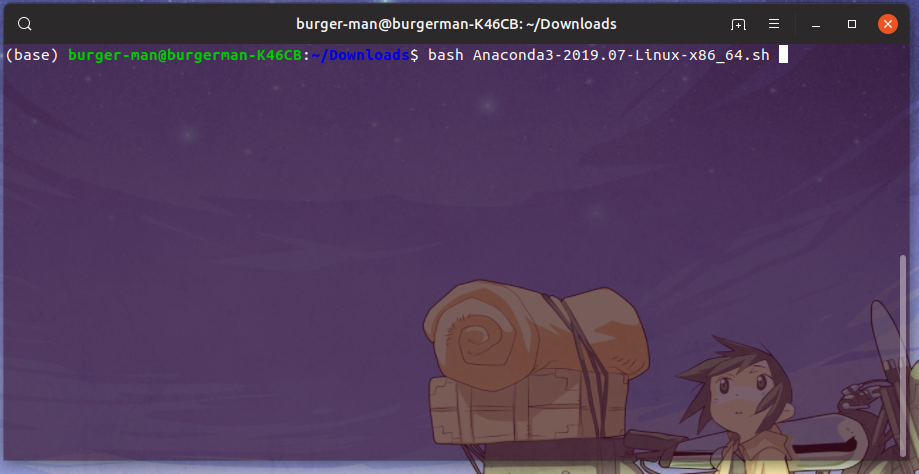
\includegraphics[width=1\textwidth]{figures/ubuntu/anacondabash.png}
\caption{Gambar install anaconda}
\label{anacondabash}
\end{figure}

\item Setelah itu, tekan \textbf{ENTER} saja seperti gambar \ref{anacondaenter}
\begin{figure}[H]
\centering
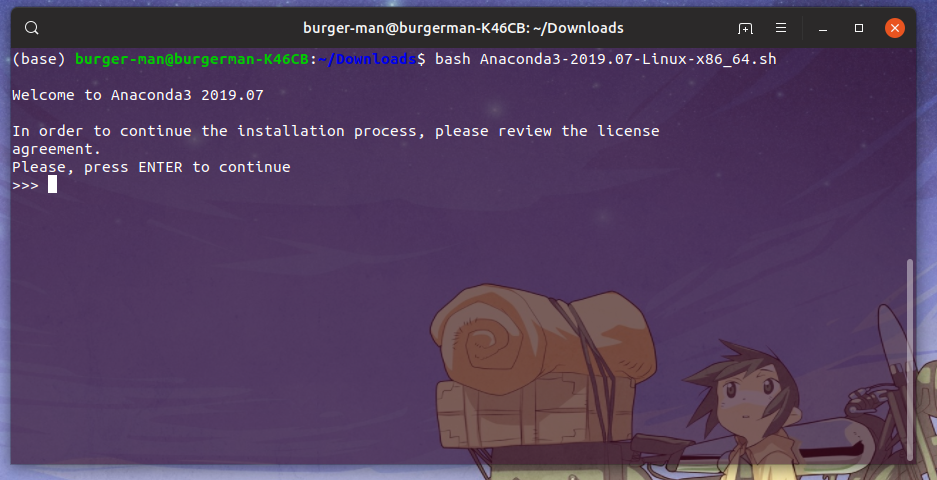
\includegraphics[width=1\textwidth]{figures/ubuntu/anacondaenter.png}
\caption{Gambar eksekusi anaconda}
\label{anacondaenter}
\end{figure}

\item Lalu akan muncul sebuah tulisan \textbf{End User License Agreement} seperti gambar \ref{entertrus}, tekan \textbf{ENTER} dan tahan hingga seperti gambar 
\begin{figure}[H]
\centering
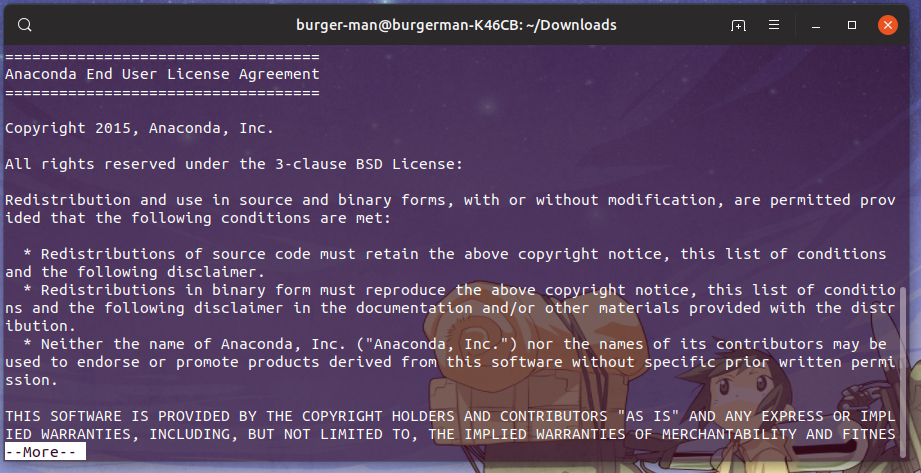
\includegraphics[width=1\textwidth]{figures/ubuntu/entertrus.png}
\caption{Gambar anaconda license agreement}
\label{entertrus}
\end{figure}
\begin{figure}[H]
\centering
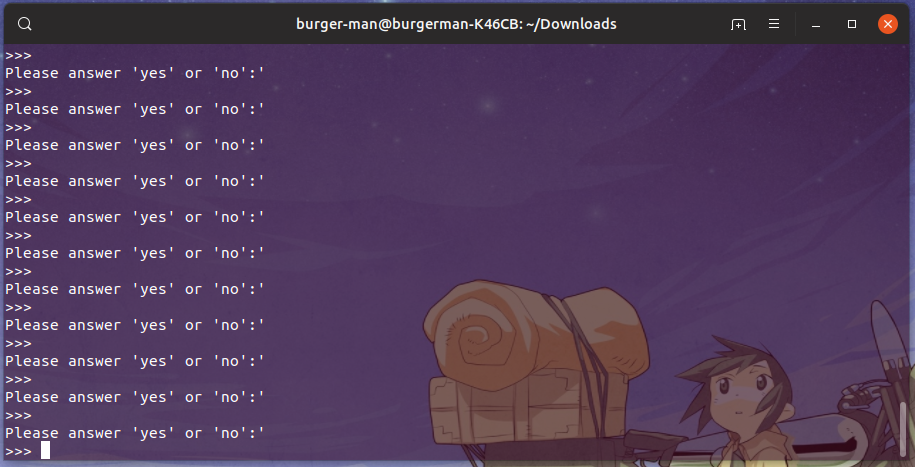
\includegraphics[width=1\textwidth]{figures/ubuntu/enterkekgini.png}
\caption{Gambar perintah yes or no}
\label{enterkekgini}
\end{figure}

\item Lalu setelah muncur perintah \textbf{\textit{'yes' or 'no'}} ketik \textbf{\textit{yes}} lalu enter

\item Setelah itu muncul path direktori instalasi anaconda kita seperti gambar \ref{enterpath} lalu tekan enter
\begin{figure}[H]
\centering
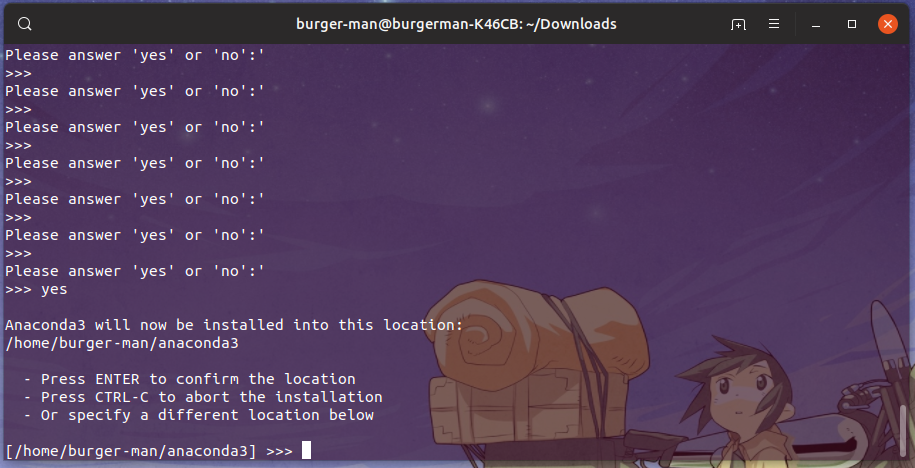
\includegraphics[width=1\textwidth]{figures/ubuntu/enterpath.png}
\caption{Gambar path anaconda}
\label{enterpath}
\end{figure}

Setelah kita selesai instalasi anaconda jangan lupa juga untuk menginstal spyder ide, caranya seperti berikut:
\begin{enumerate}

\item ketikkan perintah \textbf{\textit{sudo apt install spyder3 -y}} seperti gambar \ref{installspyder3}
\begin{figure}[H]
\centering
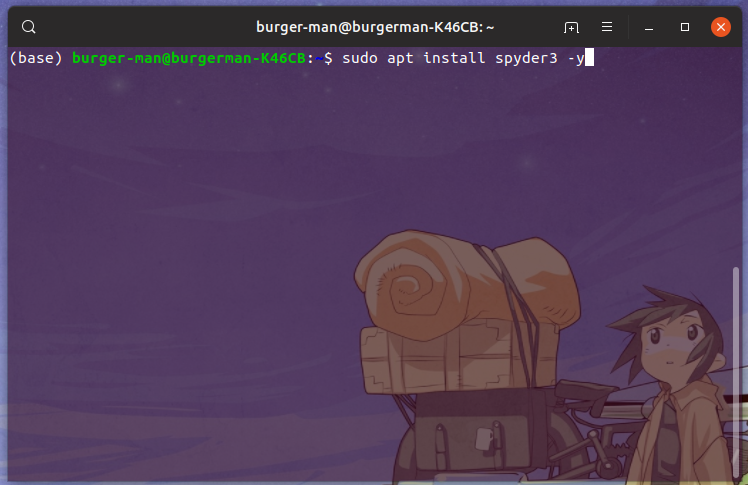
\includegraphics[width=1\textwidth]{figures/ubuntu/installspyder3.png}
\caption{Gambar perintah install spyder3}
\label{installspyder3}
\end{figure}

\item lalu jalankan dengan perintah \textbf{\textit{spyder}} atau \textbf{\textit{spyder3}}
\end{enumerate}

\end{enumerate}

\subsection{Konfigurasi \textbf{\textit{Python}}}
Setelah kita selesai instal Anaconda dan Spyder, selanjutnya kita akan mempelajari bagaimana cara setting environments python kita? caranya sebagai berikut

\begin{enumerate}

\item pertama kita buka terminal kita lalu ketikkan perintah berikut, contoh seperti gambar \ref{setpath}, lalu tekan enter
\begin{lstlisting}
export PYTHONPATH=\$PYTHONPATH:pathinstallasipythonkalian
\end{lstlisting}
\begin{figure}[H]
\centering
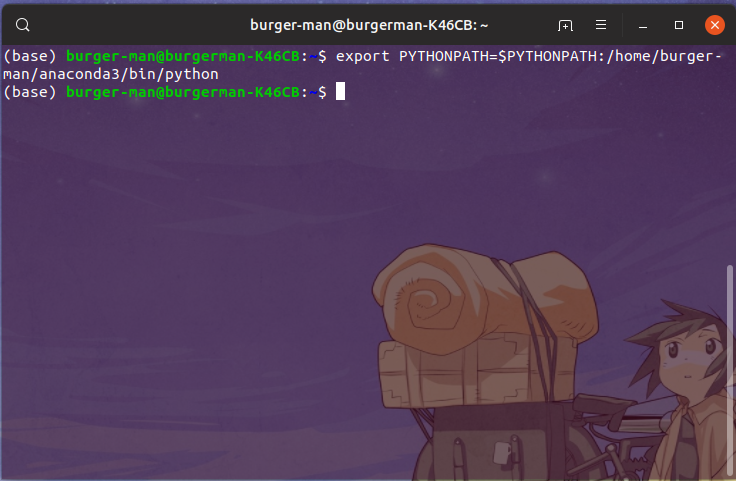
\includegraphics[width=1\textwidth]{figures/ubuntu/setpath.png}
\caption{Gambar setpath}
\label{setpath}
\end{figure}

\end{enumerate}

\section{Instalasi Pycharm}
Ikuti langkah-langkah berikut untuk install pycharm di sistem operasi windows:
\begin{enumerate}
\item Download Installer Pycharm dari situs resminya yaitu \\  \url{https://www.jetbrains.com/pycharm/download}.
\item Jalankan Installer PyCharm yang telah selesai di download, kemudian klik Next untuk melanjutkan installasi seperti pada contoh gambar \ref{installpycharm}.
\begin{figure}[H]
\centering
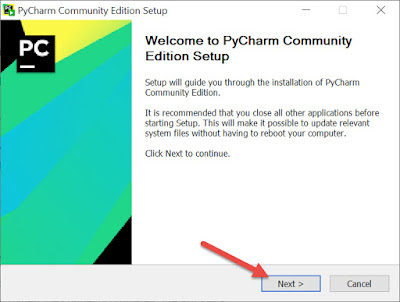
\includegraphics[scale=.65]{figures/install_pycharm1}
\caption{Klik Next untuk Install Pycharm}
\label{installpycharm}
\end{figure}
\item Tentukan destination folder jika diperlukan, atau dibiarkan default kemudian klik Next.
\begin{figure}[H]
\centering
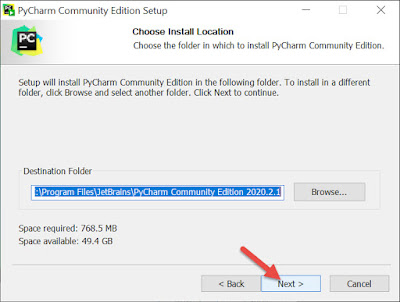
\includegraphics[scale=.65]{figures/install_pycharm2}
\caption{Menentukan lokasi folder dan klik next}
\label{installpycharm1}
\end{figure}
\item Checklist pada "Add launchers dir to PATH" kemudian klik Next.
\begin{figure}[H]
\centering
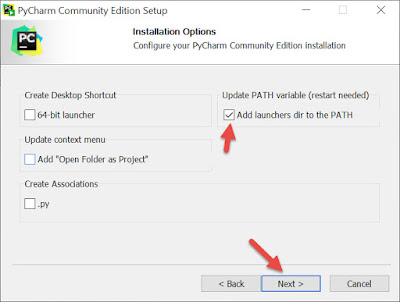
\includegraphics[scale=.65]{figures/install_pycharm3}
\caption{Add launchers dir to PATH}
\label{installpycharm3}
\end{figure}
\item Klik Install untuk melanjutkan
\begin{figure}[H]
\centering
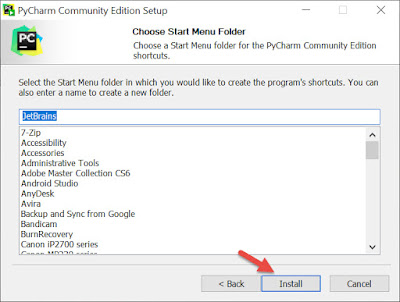
\includegraphics[scale=.65]{figures/install_pycharm4}
\caption{Klik Install}
\label{installpycharm4}
\end{figure}
\item Tunggu proses installasi PyCharm sampai selesai.
\begin{figure}[H]
\centering
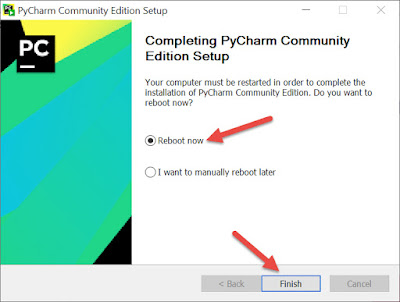
\includegraphics[scale=.65]{figures/install_pycharm6}
\caption{Reboot Now}
\label{installpycharm6}
\end{figure}
\item Setelah proses installasi PyCharm selesai, klik Reboot now, lalu klik Finish.
\end{enumerate}

\section{Membuat Akun Github}
Github merupakan software developer untuk menyimpan dan sharing project-project yang bersifat opensource, karena bersifat opensource maka project tersebut dapat dikembangkan oleh programmer lain yang ingin berkontribusi pada project, sangat bagus untuk project yang dikembangkan oleh team maupun individu. 

Github memiliki banyak keunggulan diantaranya sebagai tempat menyimpan backup project, adanya free hosting, memudahkan developer, mendukung semua bahasa pemrograman dan github juga berguna sebagai tempat penyimpanan project secara gratis.

Berikut tata cara membuat akun github:
\begin{enumerate}
\item buka browser kemudian kunjungi situs github.
\item kliktombol sign up
\begin{figure}[H]
\centering

\includegraphics[scale=.25]{figures/daftar}
\caption{Sign Up | sumber: https://omcyber.com/cara-membuat-akun-github/}
\label{git2}
\end{figure}
\item isi formulir data diri seperti username, email, password, dan verify your account. Pastikan data yang diisikan benar.
\begin{figure}[H]
\centering
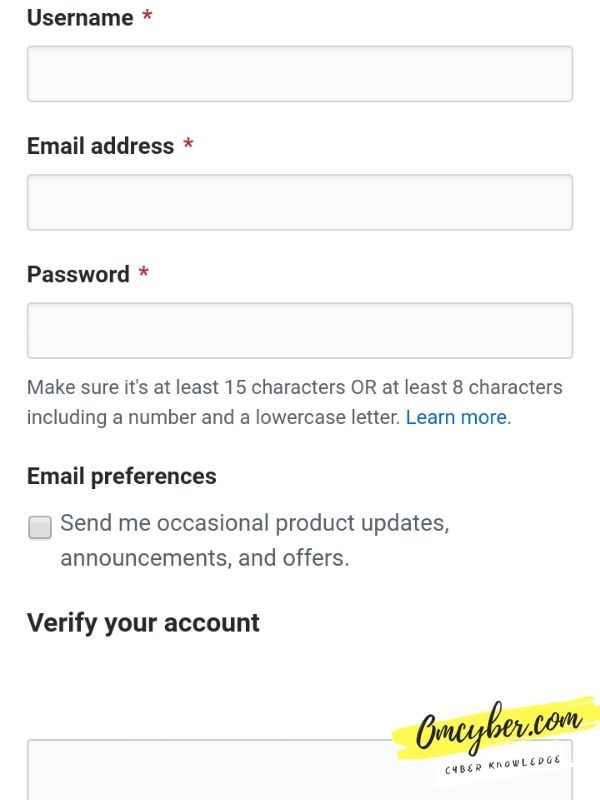
\includegraphics[scale=.25]{figures/form}
\caption{Form Daftar}
\label{git3}
\end{figure}
\item klik tombol create an account untuk membuat akun baru github.
\item silahkan pilih free plan dengan klik tombol jon a free plan
\begin{figure}[H]
\centering

\includegraphics[scale=.25]{figures/free}
\caption{Free Plan}
\label{git4}
\end{figure}
\item verifikasi email agar akun github terverifikasi
\begin{figure}[H]
\centering
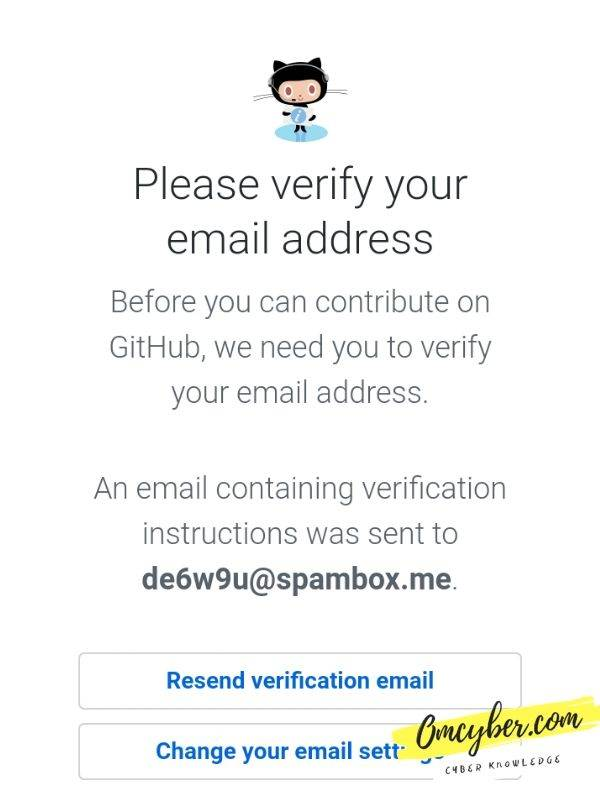
\includegraphics[scale=.25]{figures/verifikasi}
\caption{Verifikasi Email}
\label{git5}
\end{figure}
\item buka inbox email yang didaftarkan, buka email dari github dan klik verifikasi email address.
\begin{figure}[H]
\centering
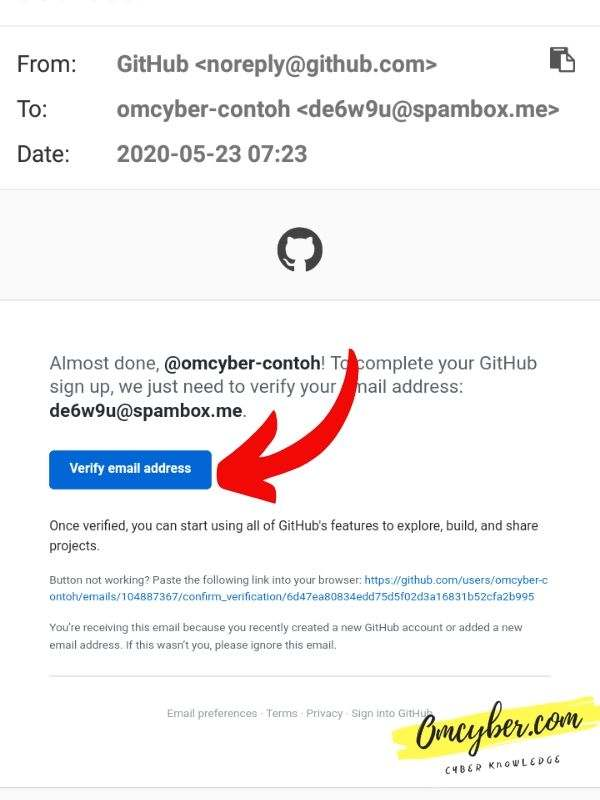
\includegraphics[scale=.25]{figures/email}
\caption{Verifikasi Email Address}
\label{git5}
\end{figure}
\item setelah berhasil verifikasi email maka akun github telah berhasil dibuat dan terverifikasi.
\begin{figure}[H]
\centering
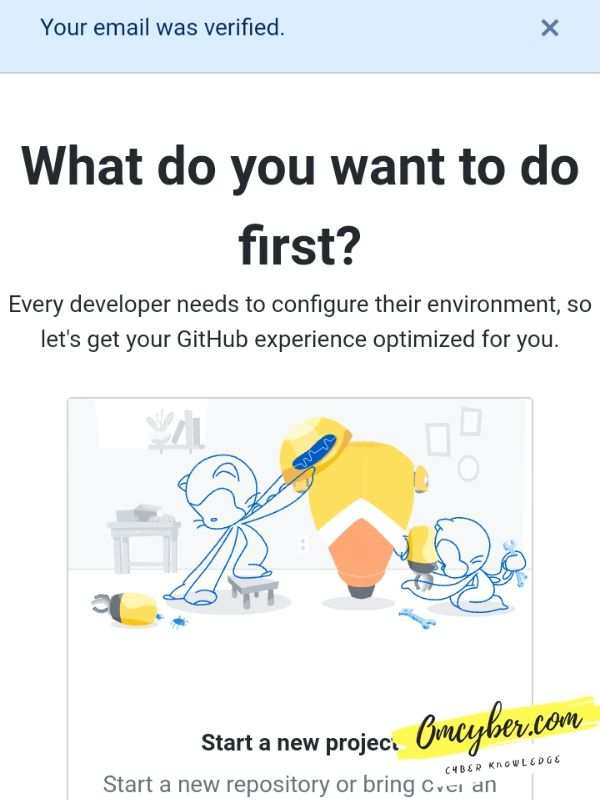
\includegraphics[scale=.25]{figures/berhasil}
\caption{Verifikasi Email Berhasil}
\label{git6}
\end{figure}
\end{enumerate}

\section{Download dan Install Git}
Sebelum melakukan instalasi git, kita memerlukan file instalasi git terlebih dahulu. File ini bisa teman-teman dapatkan dengan mengunduh file dari situs resmi git, berikut link yang dapat teman-teman kunjungi \\ \url{https://git-scm.com/downloads}. Download file yang sesuai dengan sistem operasi pada komputer teman-teman. Jika komputer teman-teman memiliki sistem operasi Windows 64bit maka teman-teman harus mengunduh file instalasi git untuk windows 64bit. Ikuti tahapan berikut untuk melakukan instalasi git:
\begin{enumerate}
\item Buka file instalasi git yang telah di download, kemudian klik next.
\begin{figure}[H]
\centering
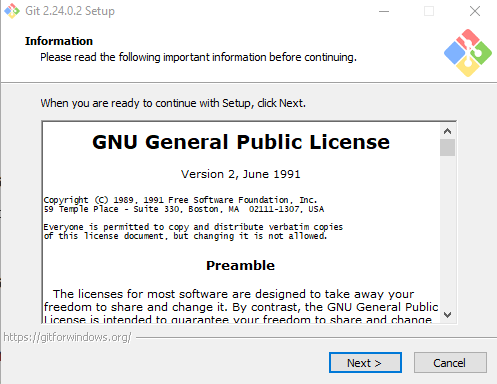
\includegraphics[scale=.5]{figures/install_git1}
\caption{Install Git}
\label{install_git1}
\end{figure}

\item Pilih lokasi instalasi git, disarankan install pada lokasi seperti gambar
\begin{figure}[H]
\centering
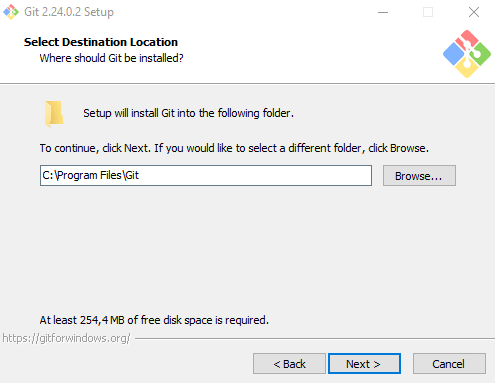
\includegraphics[scale=.5]{figures/install_git2}
\caption{Lokasi Instalasi Git}
\label{install_git2}
\end{figure}

\item Selanjutnya pilih komponen tambahan untuk install git, sesuaikan dengan kebutuhan teman-teman. Jika sudah maka klik next untuk melanjutkan instalasi.
\begin{figure}[H]
\centering
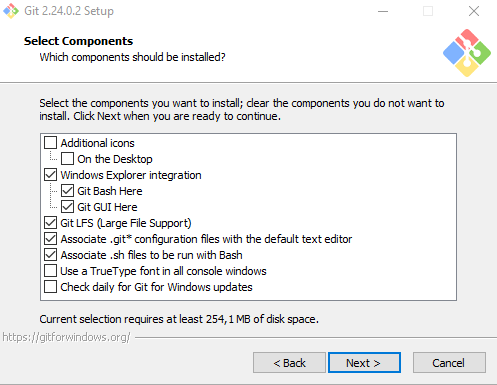
\includegraphics[scale=.5]{figures/install_git3}
\caption{Komponen Tambahan}
\label{install_git3}
\end{figure}

\item Tentukan nama aplikasi git, untuk memudahkan pencarian aplikasi maka disarankan menggunakan nama Git saja.
\begin{figure}[H]
\centering
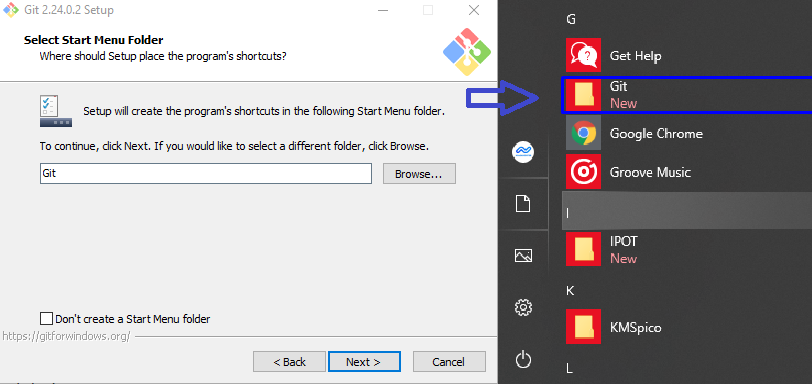
\includegraphics[scale=.35]{figures/install_git4}
\caption{Select Start Menu Folder}
\label{install_git4}
\end{figure}

\item pilih file editor untuk dikombinasikan dengan git, pada tutorial ini saya menggunakan vim editor lalu pilih next.
\begin{figure}[H]
\centering
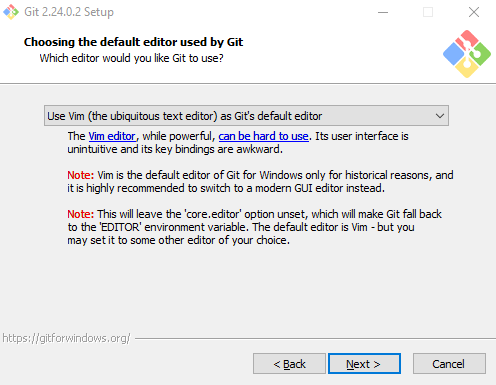
\includegraphics[scale=.5]{figures/install_git5}
\caption{Choose Default Editor}
\label{install_git5}
\end{figure}

\item selanjutnya kita perlu mengatur path environment, Pilih Git from the command line and also from 3rd-party software agar saat menjalankan perintah Git dapat dikenali di Command Prompt (CMD) pada Windows.
\begin{figure}[H]
\centering
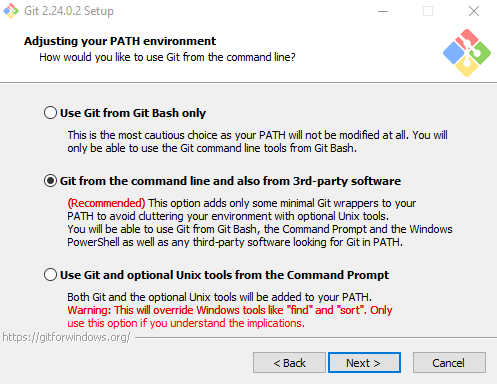
\includegraphics[scale=.5]{figures/install_git6}
\caption{PATH Environment}
\label{install_git6}
\end{figure}

\item kemudian pilih aplikasi SSH, pada tutorial ini saya memilih Use OpenSSH yang merupakan aplikasi default SSH dari Git lalu klik next.
\begin{figure}[H]
\centering
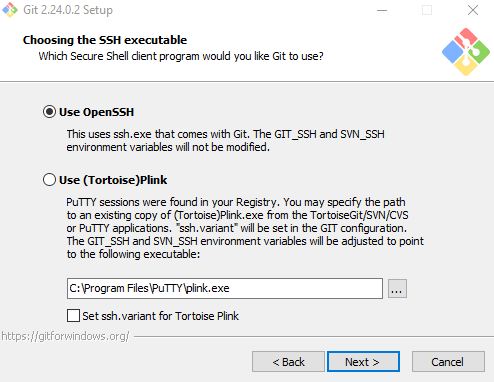
\includegraphics[scale=.5]{figures/install_git7}
\caption{Choose SSH}
\label{install_git7}
\end{figure}

\item selanjutnya pilih Checkout Windows-style, commit Unix-style line endings dan klik next
\begin{figure}[H]
\centering
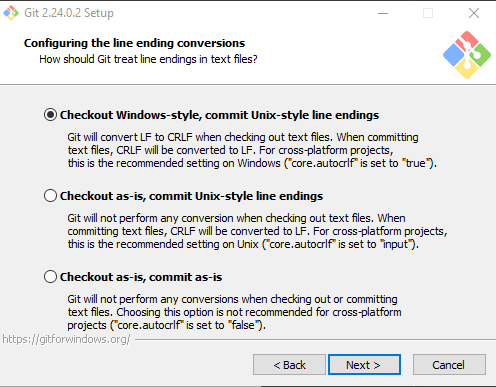
\includegraphics[scale=.5]{figures/install_git8}
\caption{Configuring the line ending}
\label{install_git8}
\end{figure}

\item pilih Use Windows’ default console windows kemudian klik next
\begin{figure}[H]
\centering
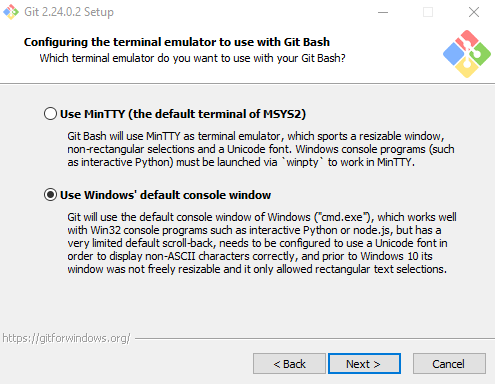
\includegraphics[scale=.5]{figures/install_git9}
\caption{Configuring the terminal emulator}
\label{install_git9}
\end{figure}

\item pilih opsi ekstra yaitu Enable File System Caching agar Git memiliki fungsi system caching dan Enable Git Credential Manager agar Git bisa dikombinasikan dengan aplikasi lain seperti Visual Studio, Android Studio, dan GitHub. Selanjutnya klik next.
\begin{figure}[H]
\centering
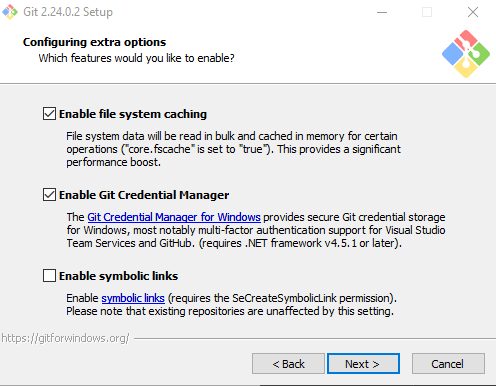
\includegraphics[scale=.5]{figures/install_git10}
\caption{Configuring extra options}
\label{install_git10}
\end{figure}

\item setelah menambahkan konfigurasi ekstra maka teman-teman bisa melakukan instalasi git dengan klik install.
\begin{figure}[H]
\centering
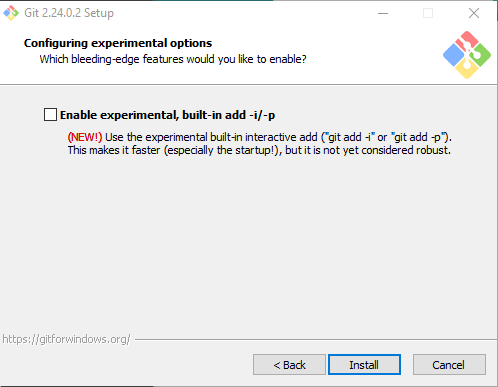
\includegraphics[scale=.5]{figures/install_git11}
\caption{Install}
\label{install_git11}
\end{figure}

\item Tunggu hingga proses instalasi selesai.
\begin{figure}[H]
\centering
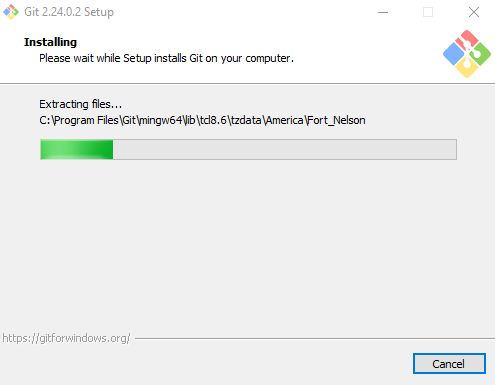
\includegraphics[scale=.5]{figures/install_git12}
\caption{Proses Install}
\label{install_git12}
\end{figure}

\item Jika instalasi telah selesai maka teman-teman bisa cek versi git untuk memastikan apakah git telah berhasil terinstal di komputer teman-teman dengan membuka command prompt atau cmd.
\begin{figure}[H]
\centering
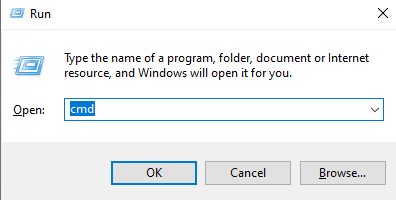
\includegraphics[scale=.5]{figures/install_git13}
\caption{Command Prompt (CMD)}
\label{install_git13}
\end{figure}

\item ketikkan perintah git --version lalu tekan enter untuk melihat versi git yang telah teman-teman install.
\begin{figure}[H]
\centering
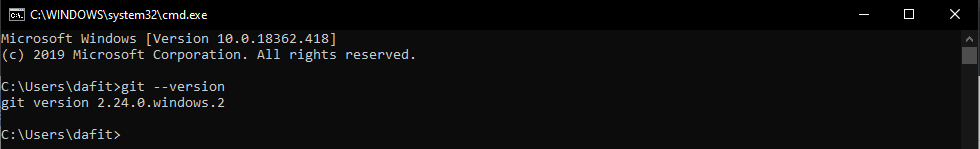
\includegraphics[scale=.35]{figures/install_git14}
\caption{Versi Git}
\label{install_git14}
\end{figure}

\end{enumerate}

\section{Konfigurasi Git}
Berikut hal yang perlu teman-teman lakukan apabila telah install git di komputer, teman-teman perlu melakukan konfigurasi email dan username akun git teman-teman. Ikuti tahapan berikut untuk melakukan konfigurasi git:
\begin{enumerate}
\item Konfigurasikan email dan username git yang telah teman-teman daftarkan pada github dengan mengetikkan perintah
\begin{verbatim}
git config --global user.name "username anda"
git config --global user.email "email_anda@gmail.com"
\end{verbatim}
\begin{figure}[H]
\centering
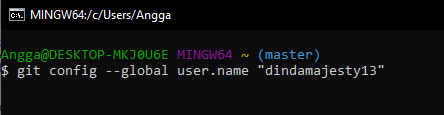
\includegraphics[scale=.75]{figures/konfig_git1}
\caption{Konfigurasi Username Git}
\label{konfig_git1}
\end{figure}

\begin{figure}[H]
\centering
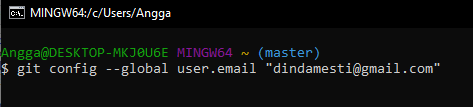
\includegraphics[scale=.75]{figures/konfig_git2}
\caption{Konfigurasi Email Git}
\label{konfig_git2}
\end{figure}

\item membuat ssh key dengan mengetikkan perintah
\begin{verbatim}
ssh-keygen -t rsa -b 4096 -C "email_anda@gmail.com"
\end{verbatim}
lalu tekan enter sebanyak tiga kali, pertama untuk membuat direktori penyimpanan ssh, kedua dan ketiga untuk menambahkan passphrase.
\begin{figure}[H]
\centering
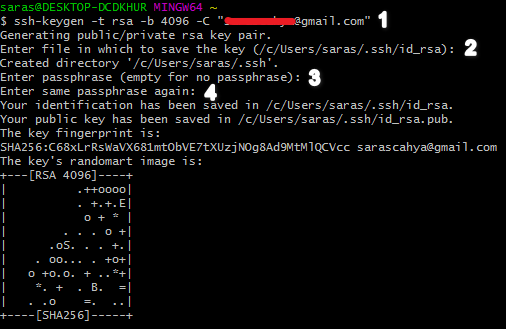
\includegraphics[scale=.75]{figures/konfig_git3}
\caption{Generate SSH key}
\label{konfig_git3}
\end{figure}

\item jika ssh key telah berhasil digenerate, ketikkan perintah
\begin{verbatim}
cd .ssh/
ls
\end{verbatim}
perintah ini digunakan untuk berpindah direktori ke direktori ssh dan menampilkan list file yang ada didalam direktori tersebut.
\begin{figure}[H]
\centering
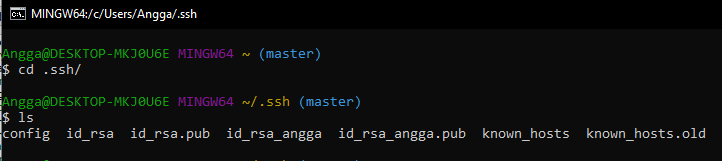
\includegraphics[scale=.5]{figures/konfig_git4}
\caption{Direktori SSH}
\label{konfig_git4}
\end{figure}

\item ketikkan perintah berikut untuk menampilkan ssh yang telah digenerate, kemudian copy ssh key yang tampil dilayar teman-teman.
\begin{verbatim}
cat id_rsa.pub
\end{verbatim}

\begin{figure}[H]
\centering
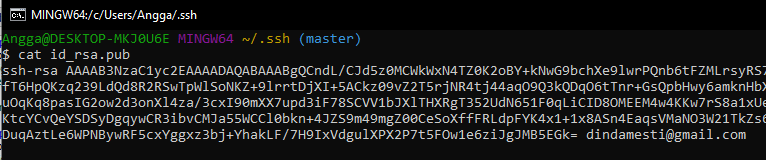
\includegraphics[scale=.5]{figures/konfig_git5}
\caption{SSH Key}
\label{konfig_git5}
\end{figure}

\item pilih menu SSH dan GPG keys
\begin{figure}[H]
\centering
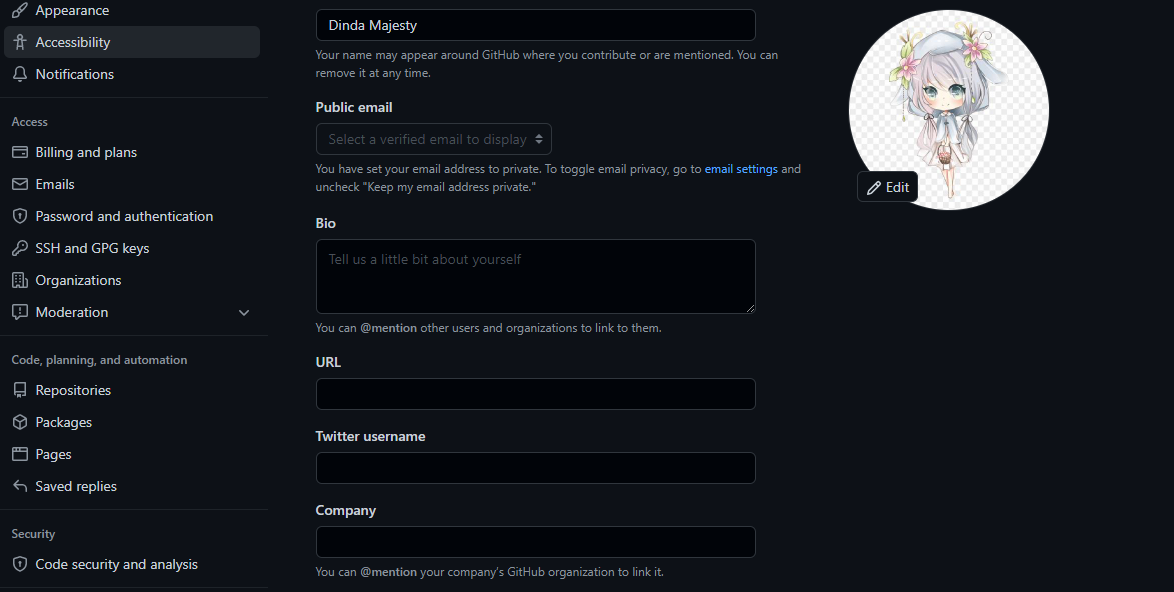
\includegraphics[scale=.35]{figures/konfig_git7}
\caption{Menu  SSH dan GPG keys}
\label{konfig_git7}
\end{figure}

\item klik tombol New SSH key
\begin{figure}[H]
\centering
\includegraphics[scale=.35]{figures/konfig_git8}
\caption{New SSH key}
\label{konfig_git8}
\end{figure}

\item isikan title, pada bagian key paste ssh key yang telah di copy sebelumnya dan klik add SSH key
\begin{figure}[H]
\centering
\includegraphics[scale=.5]{figures/konfig_git9}
\caption{Add SSH key}
\label{konfig_git9}
\end{figure}

\item sekarang teman-teman telah berhasil menambahkan ssh key pada akun github teman-teman. Selanjutnya teman-teman dapat mengklon Real-Time-Voice-Cloning project.

\end{enumerate}

\section{Fork dan Clone Voice Cloning Repositori}
berikut tutorial clone repo voice cloning menggunakan github:
\begin{enumerate}
\item Kunjungi link berikut \\ \url{https://github.com/dindamajesty13/Real-Time-Voice-Cloning}
\item Klik fork, maka repo Real-Time-Voice-Cloning akan ada di github anda.
\begin{figure}[H]
\centering
\includegraphics[scale=.3]{figures/repo}
\caption{Fork Repositori}
\label{repo1}
\end{figure}

\item buka project Real-Time-Voice-Cloning yang ada direpo anda lalu klik pada bagian code.
\begin{figure}[H]
\centering
\includegraphics[scale=.3]{figures/repo1}
\caption{Klik Tombol Code}
\label{repo2}
\end{figure}

\item pilih HTTPS dan salin url yang ada dibawah tulisan HTTPS
\begin{figure}[H]
\centering
\includegraphics[scale=.75]{figures/repo3}
\caption{Copy Url}
\label{repo3}
\end{figure}

\item buka gitbash kemudian ketikkan git clone lalu paste url yang telah di copy sebelumnya.
\begin{figure}[H]
\centering
\includegraphics[scale=.4]{figures/repo4}
\caption{Git Clone Repositori}
\label{repo4}
\end{figure}

\item Lalu tekan enter pada keyboard, tunggu hingga proses clone selesai.
\begin{figure}[H]
\centering
\includegraphics[scale=.4]{figures/repo5}
\caption{Proses Clone Repositori}
\label{repo5}
\end{figure}

\item jika proses clone telah selesai, buka pycharm.

\item klik menu file, pilih open.
\begin{figure}[H]
\centering
\includegraphics[scale=.2]{figures/repo6}
\caption{Pycharm}
\label{repo6}
\end{figure}

\item cari folder Real-Time-Voice-Cloning, kemudian klik ok
\begin{figure}[H]
\centering
\includegraphics[scale=.55]{figures/repo7}
\caption{Lokasi Folder Repositori}
\label{repo7}
\end{figure}

\item pycharm akan membuka file project Real-Time-Voice-Cloning, jika terdapat pop up create virtual environment klik ok jika versi python sama dengan 3.7, jika versi python 3.9 seperti gambar \ref{repo8} maka klik cancel dan ikuti tahapan Menambahkan Interpreter ke dalam Voice Cloning Project dibawah.
\begin{figure}[H]
\centering
\includegraphics[scale=.55]{figures/repo8}
\caption{Pop Up Create Virtual Environment}
\label{repo8}
\end{figure}

\item jika berhasil maka anda akan melihat tampilan seperti pada gambar \ref{repo9}
\begin{figure}[H]
\centering
\includegraphics[scale=.3]{figures/repo9}
\caption{Real-Time-Voice-Cloning project}
\label{repo9}
\end{figure}

\end{enumerate}

\section{Menambahkan Interpreter ke dalam Voice Cloning Project} 
Sebelum menjalankan project menggunakan Pycharm kita membutuhkan interpreter, saya menyarankan untuk menggunakan virtual environment atau conda environment jika anda pengguna anaconda. Dalam pembuatan interpreter penggunaan python 3.7 sangat direkomendasikan karena pada pembuatan voice cloning ini menggunakan tensorflow versi 1.x sehingga teman-teman harus mendownload python versi 3.7, ffmpeg, pytorch, dan requirements.
Berikut tata pembuatan virtual environment untuk project voice cloning ini:

\subsection{Download dan Install Python 3.7}
\begin{enumerate}
\item download python versi 3.7 pada website resmi python atau kunjungi link berikut \url{https://www.python.org/downloads/release/python-371/}

\item Pilih file yang sesuai dengan sistem operasi dan processor pada komputer teman-teman.
\begin{figure}[H]
\centering
\includegraphics[scale=.35]{figures/python1}
\caption{Download Python 3.7}
\label{python1}
\end{figure}

\item Centang add python 3.7 to PATH agar python yang diinstal ditambahkan ke environment variabel komputer teman-teman, kemudian klik install now.
\begin{figure}[H]
\centering
\includegraphics[scale=.4]{figures/python2}
\caption{Add Python to PATH}
\label{python2}
\end{figure}

\item Jika instalasi telah selesai maka teman-teman akan melihat tampilan seperti gambar \ref{python3}
\begin{figure}[H]
\centering
\includegraphics[scale=.4]{figures/python3}
\caption{Success Install Python 3.7}
\label{python3}
\end{figure}

\item Untuk memastikan apakah python 3.7 telah benar-benar berhasil terinstal teman-teman dapat melakukan pengecekan melalui command prompt (CMD) dengan mengetikkan perintah python kemudian tekan enter.
\begin{figure}[H]
\centering
\includegraphics[scale=.4]{figures/python4}
\caption{Check Python Version}
\label{python4}
\end{figure}

\end{enumerate}

\subsection{Download dan Install FFmpeg}

\begin{enumerate}

\item Setelah menginstal python 3.7, kita harus menginstal ffmpeg, kunjungi link berikut untuk mendapatkan file instalasi ffmpeg \url{https://ffmpeg.org/download.html}. Sesuaikan file download dengan sistem operasi yang teman-teman gunakan. Pada tutorial ini saya menggunalan system operasi windows.
\begin{figure}[H]
\centering
\includegraphics[scale=.35]{figures/python5}
\caption{Download FFmpeg}
\label{python5}
\end{figure}

\item Pilih Windows builds from gyan.dev. Kemudian teman-teman akan diarahkan ke halaman seperti pada gambar \ref{python6}
\begin{figure}[H]
\centering
\includegraphics[scale=.4]{figures/python6}
\caption{Download FFmpeg for Windows}
\label{python6}
\end{figure}

\item Download file ffmpeg-git-full.7z kemudian extract file instalasi FFmpeg yang telah didownload.
\begin{figure}[H]
\centering
\includegraphics[scale=1.5]{figures/python7}
\caption{Extract File Instalasi}
\label{python7}
\end{figure}

\item Ganti nama direktori menjadi FFmpeg
\begin{figure}[H]
\centering
\includegraphics[scale=1.5]{figures/python8}
\caption{Ganti Nama Folder}
\label{python8}
\end{figure}

\item Copy folder dan Paste folder ke Local Disk C
\begin{figure}[H]
\centering
\includegraphics[scale=1.5]{figures/python10}
\caption{Move Folder}
\label{python10}
\end{figure}

\item Klik start menu pada komputer anda lalu ketikkan environment variable. Klik edit environment variables for your account
\begin{figure}[H]
\centering
\includegraphics[scale=1.5]{figures/python10}
\caption{Move Folder}
\label{python10}
\end{figure}

\item Klik menu environment variables
\begin{figure}[H]
\centering
\includegraphics[scale=1.5]{figures/python11}
\caption{Environment Variables}
\label{python11}
\end{figure}

\item Pada bagian PATH klik edit maka pop up window edit environment variable seperti pada gambar \ref{python12} akan muncul. Ketikkan lokasi folder bin FFmpeg lalu klik OK.
\begin{verbatim}
 C:\ffmpeg\bin
\end{verbatim}

\begin{figure}[H]
\centering
\includegraphics[scale=1.1]{figures/python12}
\caption{Add FFmpeg to PATH}
\label{python12}
\end{figure}

\item Klik OK untuk menyimpan perubahan pada environment variables
\begin{figure}[H]
\centering
\includegraphics[scale=1.2]{figures/python13}
\caption{Save Changes}
\label{python13}
\end{figure}

\item Untuk melakukan pengecekan apakah FFmpeg telah berhasil di install pada komputer, teman-teman bisa melakukan pengecekan dengan mengetikkan ffmpeg -version pada command prompt.
\begin{figure}[H]
\centering
\includegraphics[scale=.35]{figures/python14}
\caption{Check FFmpeg Version}
\label{python14}
\end{figure}

\end{enumerate}

\subsection{Tutorial Membuat Virtual Environment}
Berikut tutorial membuat virtual environment menggunakan pycharm dan python 3.7:
\begin{enumerate}

\item Buka settings pycharm dengan mengklik menu file lalu pilih settings. Pada menu Project Real-Time-Voice-Cloning pilih menu python interpreter.
\begin{figure}[H]
\centering
\includegraphics[scale=.4]{figures/env1}
\caption{Menu Settings Python Interpreter}
\label{env1}
\end{figure}

\item Klik No interpreter lalu pilih show all maka akan muncul python interpreter seperti pada gambar \ref{env2}. Klik tanda tambah untuk membuat interpreter baru.
\begin{figure}[H]
\centering
\includegraphics[scale=.4]{figures/env2}
\caption{Python Interpreter}
\label{env2}
\end{figure}

\item Pilih Virtual Environment, lalu pilih New Environment, isikan lokasi tempat environment disimpan dan isikan file exe python 3.7  pada base interpreter. Lalu klik OK.
\begin{figure}[H]
\centering
\includegraphics[scale=.4]{figures/env3}
\caption{Add Python Interpreter}
\label{env3}
\end{figure}

\item Tunggu hingga proses creating virtual environment selesai.
\begin{figure}[H]
\centering
\includegraphics[scale=.4]{figures/env4}
\caption{Creating Virtual Environment}
\label{env4}
\end{figure}

\item Pilih virtual environment yang telah kita buat lalu klik OK.
\begin{figure}[H]
\centering
\includegraphics[scale=.4]{figures/env5}
\caption{Pilih Virtual Environment}
\label{env5}
\end{figure}

\item Berikut tampilan virtual environment yang telah kita buat menggunakan python 3.7.
\begin{figure}[H]
\centering
\includegraphics[scale=.4]{figures/env6}
\caption{Apply Virtual Environment}
\label{env6}
\end{figure}

\item Pada kanan bawah pycharm teman-teman akan melihat progress bar yang menandakan pycharm sedang melakukan inisialisasi terhadap virtual environment teman-teman. Jalankan program apabila proses tersebut telah selesai.
\begin{figure}[H]
\centering
\includegraphics[scale=.4]{figures/env7}
\caption{Inisialisasi Virtual Environment}
\label{env7}
\end{figure}

\end{enumerate}

\subsection{Tutorial Membuat Conda Environment}
Berikut tutorial membuat conda environment menggunakan pycharm dan python 3.7:
\begin{enumerate}

\item Buka settings pycharm dengan mengklik menu file lalu pilih settings. Pada menu Project Real-Time-Voice-Cloning pilih menu python interpreter.
\begin{figure}[H]
\centering
\includegraphics[scale=.4]{figures/cenv1}
\caption{Menu Settings Project}
\label{cenv1}
\end{figure}

\item Klik No interpreter lalu pilih show all maka akan muncul python interpreter seperti pada gambar \ref{cenv2}. Klik tanda tambah untuk membuat interpreter baru.
\begin{figure}[H]
\centering
\includegraphics[scale=.4]{figures/cenv2}
\caption{Show All Interpreter}
\label{cenv2}
\end{figure}

\item Pilih Conda Environment, lalu pilih New Environment.
\begin{figure}[H]
\centering
\includegraphics[scale=.4]{figures/cenv3}
\caption{Conda Environment}
\label{cenv3}
\end{figure}

\item Isikan lokasi tempat conda environment disimpan, pilih python version 3.7  dan isikan lokasi file conda.exe pada conda executable. Lalu klik OK. 
\begin{figure}[H]
\centering
\includegraphics[scale=.4]{figures/cenv4}
\caption{Create New Conda Environment}
\label{cenv4}
\end{figure}

\item Tunggu hingga proses pembuatan conda environment selesai. 
\begin{figure}[H]
\centering
\includegraphics[scale=.4]{figures/cenv5}
\caption{Creating Conda Environment}
\label{cenv5}
\end{figure}

\item Berikut tampilan conda environment yang telah kita buat, klik Apply lalu klik OK.
\begin{figure}[H]
\centering
\includegraphics[scale=.4]{figures/cenv6}
\caption{Apply Conda Environment}
\label{cenv6}
\end{figure}

\item Tunggu hingga proses inisialisasi conda environment selesai, jika sudah teman-teman bisa menginstalkan requirements yang teman-teman gunakan dan menjalankan program yang ingin dijalankan.
\begin{figure}[H]
\centering
\includegraphics[scale=.4]{figures/cenv7}
\caption{Progress Bar Inisialisasi Conda Environment}
\label{cenv7}
\end{figure}

\end{enumerate}

\subsection{Install Requirements}
Perhatikan struktur folder project voice cloning teman-teman maka akan terlihat file dengan nama requirements.txt, file tersebut berisikan library-library yang digunakan dalam project ini. Library tersebut harus diinstall terlebih dahulu agar project dapat dijalankan dengan baik. Berikut tata cara instalasi requirements:
\begin{enumerate}
\item Jika teman-teman menggunakan conda environment maka buka anaconda prompt dan ketikkan perintah berikut untuk pindah directory dan mengaktifkan conda environment:
\begin{lstlisting}
cd ProgramData/Anaconda3/envs
conda activate your_environment
\end{lstlisting}

\begin{figure}[H]
\centering
\includegraphics[scale=.4]{figures/req4}
\caption{Activate Conda Environment}
\label{req4}
\end{figure}

\item Ketikkan perintah berikut untuk menginstal pip, tunggu hingga proses instalasi selesai.
\begin{lstlisting}
conda install -c anaconda pip
\end{lstlisting}

\begin{figure}[H]
\centering
\includegraphics[scale=.4]{figures/req5}
\caption{Install Pip using Anaconda Prompt}
\label{req5}
\end{figure}

\item Ketikkan perintah berikut untuk menginstal requirements, tunggu hingga proses instalasi selesai.
\begin{lstlisting}
pip install -r C:\Users\Angga\Real-Time-Voice-Cloning\requirements.txt
\end{lstlisting}

\begin{figure}[H]
\centering
\includegraphics[scale=.4]{figures/req6}
\caption{Install Requirements using Anaconda Prompt}
\label{req6}
\end{figure}

\item Pastikan requirements telah terinstall, buka python interpreter untuk melakukan pengecekan.

\begin{figure}[H]
\centering
\includegraphics[scale=.4]{figures/req7}
\caption{Sukses Install Requirements pada Conda Environment}
\label{req7}
\end{figure}

\item Jika teman-teman menggunakan virtual environment maka buka command prompt dan ketikkan perintah berikut untuk pindah directory dan mengaktifkan virtual environment:
\begin{lstlisting}
cd your-project
.\venv\Scripts\activate
\end{lstlisting}

\begin{figure}[H]
\centering
\includegraphics[scale=.4]{figures/req1}
\caption{Activate Virtual Environment with Command Prompt}
\label{req1}
\end{figure}

\item Ketikkan perintah berikut untuk menginstal requirements, tunggu hingga proses instalasi selesai.
\begin{lstlisting}
pip install -r requirements.txt
\end{lstlisting}

\begin{figure}[H]
\centering
\includegraphics[scale=.4]{figures/req2}
\caption{Install Requirements using Command Prompt}
\label{req2}
\end{figure}

\item Pastikan semua library yang dibutuhkan telah terinstall, buka Settings lalu ke menu python interpreter maka teman-teman akan melihat library yang telah berhasil diinstall pada interpreter teman-teman seperti pada gambar \ref{req3}

\begin{figure}[H]
\centering
\includegraphics[scale=.4]{figures/req3}
\caption{Berhasil Install Requirement pada Virtual Environment}
\label{req3}
\end{figure}
\end{enumerate}

\subsection{Download and install Pytorch dengan Anaconda}
Pytorch merupakan library open source yang digunakan dalam pengembangan dan pelatihan neural network. Dalam project ini, apabila komputer teman-teman memiliki GPU yang mendukung maka saya sarankan untuk menggunakan GPU dalam proses training. Tidak masalah jika tidak memiliki GPU, teman-teman dapat melakukan proses training menggunakan CPU. Instalasi Pytorch dapat dilakukan dengan cuda ataupun Pytorch dan cpu saja.

Berikut cara instalasi Pytorch:
\begin{enumerate}
\item Kunjungi situs web pytorch, berikut link website \url{https://pytorch.org/}.
\item Perhatikan gambar \ref{pytorch1}. Pastikan teman-teman memilih stable build pytorch dan menyesuaikan sistem operasi dengan komputer teman-teman. Apabila teman-teman menggunakan conda environment maka pilih conda dan bahasa pemrograman python. Jika teman-teman menggunakan GPU maka select Cuda dengan versi yang teman-teman inginkan, pilih CPU apabila menggunakan CPU. Pada run this command teman-teman akan melihat perinta instalasi menggunakan conda, lalu copy perintah tersebut.
\begin{figure}[H]
\centering
\includegraphics[scale=.35]{figures/pytorch1}
\caption{Select Pytorch with Conda}
\label{pytorch1}
\end{figure}

\item Jika teman-teman menggunakan conda environment, buka anaconda prompt, lalu ketikkan perintah berikut untuk pindah direktori.
\begin{verbatim}
cd ProgramData/Anaconda3/envs
\end{verbatim}
perintah ini untuk mengaktifkan conda environment teman-teman. Ganti your-environment dengan nama conda environment yang sebelumnya telah teman-teman buat.
\begin{verbatim}
conda activate your-environment
\end{verbatim}

\item Jika conda environment telah aktif maka teman-teman paste kan perintah yang telah di copy sebelumnya lalu tekan enter.
\begin{lstlisting}
conda install pytorch torchvision torchaudio cudatoolkit=10.2 -c pytorch
\end{lstlisting}
\begin{figure}[H]
\centering
\includegraphics[scale=.35]{figures/pytorch9}
\caption{Install Pytorch with Anaconda Prompt}
\label{pytorch9}
\end{figure}

\item Ketikkan y lalu tekan enter. Tunggu hingga proses instalasi Pytorch selesai.
\begin{figure}[H]
\centering
\includegraphics[scale=.35]{figures/pytorch8}
\caption{Proses Install Pytorch with Anaconda Prompt}
\label{pytorch8}
\end{figure}

\item Apabila instalasi telah selesai maka teman-teman bisa melakukan pengecekan pada package pytorch yang telah di install.
\begin{figure}[H]
\centering
\includegraphics[scale=.35]{figures/pytorch10}
\caption{Instalasi Pytorch Selesai}
\label{pytorch10}
\end{figure}

\item untuk memastikan apakah pytorch sudah berhasil di install maka teman-teman dapat melakukan pengecekan dengan cara mengetikkan perintah python lalu tekan enter.
\begin{figure}[H]
\centering
\includegraphics[scale=.35]{figures/pytorch11}
\caption{Check Instalasi Pytorch}
\label{pytorch11}
\end{figure}


\item Selanjutnya teman-teman ketikkan perintah import torch lalu tekan enter.
\begin{figure}[H]
\centering
\includegraphics[scale=.65]{figures/pytorch12}
\caption{Import Pytorch}
\label{pytorch12}
\end{figure}

\item Ketikkan perintah berikut untuk melihat versi pytorch yang telah berhasil di install.
\begin{verbatim}
 print(torch.__version__)
\end{verbatim}
\begin{figure}[H]
\centering
\includegraphics[scale=.5]{figures/pytorch13}
\caption{Print Pytorch Version}
\label{pytorch13}
\end{figure}

\end{enumerate}

\subsection{Download and install Pytorch dengan Pip}
Berikut cara instalasi Pytorch menggunakan pip
\begin{enumerate}
\item Kunjungi situs web pytorch, berikut link website \url{https://pytorch.org/}.

\item Perhatikan gambar \ref{pytorch2}. Pastikan teman-teman memilih stable build pytorch dan menyesuaikan sistem operasi dengan komputer teman-teman. Apabila menggunakan virtual environment maka pilih Pip lalu copy perintah pada run this command.
\begin{figure}[H]
\centering
\includegraphics[scale=.45]{figures/pytorch2}
\caption{Select Pytorch with Pip}
\label{pytorch2}
\end{figure}

\item Jika teman-teman menggunakan virtual environment, buka command prompt, lalu ketikkan perintah berikut untuk mengaktifkan virtual environment teman-teman. Ganti my-env dengan nama environment yang telah teman-teman buat sebelumnya.
\begin{verbatim}
.\my-env\Scripts\activate
\end{verbatim}

\item Jika virtual environment telah aktif maka teman-teman paste kan perintah yang telah di copy sebelumnya lalu tekan enter.
\begin{lstlisting}
pip3 install torch==1.10.2+cu102 torchvision==0.11.3+cu102 torchaudio===0.10.2+cu102 -f https://download.pytorch.org/whl/cu102/torch_stable.html
\end{lstlisting}

\begin{figure}[H]
\centering
\includegraphics[scale=.35]{figures/pytorch3}
\caption{Install Pytorch with Pip}
\label{pytorch3}
\end{figure}

\item Tunggu hingga proses instalasi Pytorch selesai. Buka python interpreter dan lihat apakah package pytorch sudah ada atau belum.
\begin{figure}[H]
\centering
\includegraphics[scale=.35]{figures/pytorch4}
\caption{Install Pytorch Berhasil}
\label{pytorch4}
\end{figure}

\item untuk memastikan apakah pytorch sudah berhasil di install maka teman-teman dapat melakukan pengecekan dengan cara mengetikkan perintah python lalu tekan enter.
\begin{figure}[H]
\centering
\includegraphics[scale=.35]{figures/pytorch5}
\caption{Check Version Pytorch}
\label{pytorch5}
\end{figure}

\item Selanjutnya teman-teman ketikkan perintah import torch lalu tekan enter.
\begin{figure}[H]
\centering
\includegraphics[scale=.35]{figures/pytorch6}
\caption{Import Torch}
\label{pytorch6}
\end{figure}

\item Ketikkan perintah berikut untuk melihat versi pytorch yang telah berhasil di install.
\begin{verbatim}
print(torch.__version__)
\end{verbatim}
\begin{figure}[H]
\centering
\includegraphics[scale=.35]{figures/pytorch7}
\caption{Print Torch Version}
\label{pytorch7}
\end{figure}

\end{enumerate}


